%%%%%%%%%%%%%%%%%%%%%%%%%%%%%%%%%%%%%%%%%
% Journal Article
% LaTeX Template
% Version 1.4 (15/5/16)
%
% This template has been downloaded from:
% http://www.LaTeXTemplates.com
%
% Original author:
% Frits Wenneker (http://www.howtotex.com) with extensive modifications by
% Vel (vel@LaTeXTemplates.com)
%
% License:
% CC BY-NC-SA 3.0 (http://creativecommons.org/licenses/by-nc-sa/3.0/)
%
%%%%%%%%%%%%%%%%%%%%%%%%%%%%%%%%%%%%%%%%%

%----------------------------------------------------------------------------------------
%	PACKAGES AND OTHER DOCUMENT CONFIGURATIONS
%----------------------------------------------------------------------------------------

\documentclass[twoside,onecolumn]{article}

\usepackage{blindtext} % Package to generate dummy text throughout this template 
\usepackage{graphicx}
\graphicspath{ {Imagenes/} }
\usepackage[sc]{mathpazo} % Use the Palatino font
\usepackage[T1]{fontenc} % Use 8-bit encoding that has 256 glyphs
\linespread{1.05} % Line spacing - Palatino needs more space between lines
\usepackage{microtype} % Slightly tweak font spacing for aesthetics

\usepackage[english]{babel} % Language hyphenation and typographical rules

\usepackage[hmarginratio=1:1,top=32mm,columnsep=20pt]{geometry} % Document margins
\usepackage[hang, small,labelfont=bf,up,textfont=it,up]{caption} % Custom captions under/above floats in tables or figures
\usepackage{booktabs} % Horizontal rules in tables

\usepackage{lettrine} % The lettrine is the first enlarged letter at the beginning of the text

\usepackage{enumitem} % Customized lists
\setlist[itemize]{noitemsep} % Make itemize lists more compact

\usepackage{abstract} % Allows abstract customization
\renewcommand{\abstractnamefont}{\normalfont\bfseries} % Set the "Resumen" text to bold
\renewcommand{\abstracttextfont}{\normalfont\small\itshape} % Set the abstract itself to small italic text

\usepackage{titlesec} % Allows customization of titles
\renewcommand\thesection{\Roman{section}} % Roman numerals for the sections
\renewcommand\thesubsection{\roman{subsection}} % roman numerals for subsections
\titleformat{\section}[block]{\large\scshape\centering}{\thesection.}{1em}{} % Change the look of the section titles
\titleformat{\subsection}[block]{\large}{\thesubsection.}{0.2em}{} % Change the look of the section titles

\usepackage{fancyhdr} % Headers and footers
\pagestyle{fancy} % All pages have headers and footers
\fancyhead{} % Blank out the default header
\fancyfoot{} % Blank out the default footer
\fancyhead[C]{Comparación de despliegue de un gestor de base de datos NoSQL mediante Docke $\bullet$ Junio 2019 $\bullet$ Trabajo Final} % Custom header text
\fancyfoot[RO,LE]{\thepage} % Custom footer text

\usepackage{titling} % Customizing the title section

\usepackage{hyperref} % For hyperlinks in the PDF

%----------------------------------------------------------------------------------------
%	TITLE SECTION
%----------------------------------------------------------------------------------------
\setlength{\droptitle}{-4\baselineskip} % Move the title up

\pretitle{\begin{center}\Huge\bfseries} % Article title formatting
\posttitle{\end{center}} % Article title closing formatting
\title{Comparación de despliegue de un gestor de base de datos NoSQL mediante Docker} % Article title
\author{%
\textsc{Marko Antonio Rivas Rios} \\[1ex] % Your name
\textsc{Jorge Luis Mamani Maquera} \\[1.01ex] % Your name
\textsc{Orlando Antonio Acosta Ortiz} \\[1.02ex] % Your name
\textsc{Yofer Nain Catari Cabrera} \\[1.03ex] % Your name
\textsc{Orestes Ramirez Ticona} \\[1.04ex] % Your name
\textsc{Roberto Zegarra Reyes} \\[1.05ex] % Your name
\normalsize Universidad Privada de Tacna \\  % Your institution
\normalsize {} % Your email address
%\and % Uncomment if 2 authors are required, duplicate these 4 lines if more
%\textsc{Jane Smith}\thanks{Corresponding author} \\[1ex] % Second author's name
%\normalsize University of Utah \\ % Second author's institution
%\normalsize \href{mailto:jane@smith.com}{jane@smith.com} % Second author's email address
}
\date{Junio 22, 2019} % Leave empty to omit a date
\renewcommand{\maketitlehookd}{%
\begin{abstract}
\noindent Docker is an open source project created in 2013 and which has been a revolution for the development and deployment of operations. Docker abstracts the host's hardware and operating system by running the applications in containers, isolated compartments that contain all the resources for an application or service.
In this work we will see how to use Docker for the development of simple applications, learning how to deploy a NOSQL database with Docker.
\end{abstract}
\begin{abstract}
\noindent Docker es un proyecto open source creado en 2013 y que ha supuesto una revolución para el desarrollo y despliegue de operaciones. Docker abstrae el hardware y el sistema operativo del host ejecutando las aplicaciones en contenedores, compartimentos aislados que contienen todos los recursos para una aplicación o servicio.

En este trabajo veremos cómo usar Docker para el desarrollo de aplicaciones sencillas, aprendiendo a desplegar una base de datos NOSQL con Docker.
\end{abstract}
}


%----------------------------------------------------------------------------------------

\begin{document}

% Print the title
\maketitle

%----------------------------------------------------------------------------------------
%	ARTICLE CONTENTS
%----------------------------------------------------------------------------------------

\section{Introducción}

\lettrine[nindent=0em,lines=2]{E}l potente concepto de Microservicios está cambiando poco a poco la industria. Grandes servicios monolíticos están dando paso lentamente al enjambre microservicios pequeños y autónomos que trabajan en conjunto. El proceso va acompañado de otra tendencia del mercado: la contenerización. Juntos, ayudan a construir sistemas  sin precedentes. La contenerización cambia no sólo la arquitectura de los servicios, sino también la estructura de ambientes utilizados para crearlos.
\textbf{}\\
Ahora, cuando el software se distribuye en contenedores, los desarrolladores tienen plena libertad para decidir qué aplicaciones necesitan. Como resultado, incluso los entornos complejos, como los servidores de grades bases de datos e infraestructura de análisis complejos pueden crear instancias en cuestión de segundos. El desarrollo de software se hace más fácil y más eficaz.

\section{Objetivos}
\begin{flushright}
\begin{itemize}
Se busca saber un poco mas sobre:
\\
%------------------------------------------------
\textbf{}\\
- Las bases de datos relacionales y no relacionales.
\textbf{}\\
- Realizar comparaciones en cuanto funcionamiento, metodologias etc.







\section{SQL y NoSQL}

\subsection{Base de datos SQL}

Structured Query language (SQL) o lenguaje de consulta estructurada, utiliza un estándar para manipular el contenido de las bases de datos relacionales. Cuenta con su propio lenguaje para consultar, insertar, actualizar y eliminar registros de la base de datos.\textbf{}\\
Se compone de una o varias tablas y cada tabla puede contener múltiples relaciones. En el siguiente elemento pongo como ejemplo en como está estructurada una sencilla base de datos por medio de tablas.
\textbf{}\\

\includegraphics[scale=0.5]{sql1}
\textbf{}\\
Las tablas representan la entidad de cada modelo de datos. Las relaciones permiten garantizar la persistencia de datos, evita la duplicidad de datos y controla la eliminación en cascada. Para ingresar un nuevo nuevo evento, bastaría con ingresar un nuevo registro en la tabla events.\textbf{}\\
SQL cuenta con un lenguaje de alto nivel que permite manipular la base de datos casi de cualquier forma. Por su manera de operar ayuda a mantener la integridad de los datos.
\textbf{}\\
\textbf{}\\
\textbf{}\\
\textbf{}\\
\textbf{}\\
\textbf{}\\
\textbf{}\\
\textbf{}\\

 Por ejemplo:
\textbf{}\\
\textbf{}\\
Para obtener la lista de todos los deportes
SELECT id, name FROM sports
\textbf{}\\
\textbf{Ingresar varios registros a la tabla categoría}\\
\textbf{}\\
INSERT INTO categories VALUES (Varonil, Femenil, mixto)
\textbf{}\\
\textbf{Su uso es más frecuente es en sistemas donde se necesite cuidar la integridad de datos como los bancos, sistemas de ventas, hospitales, CMS como WordPress.}\\
\textbf{}\\
\textbf{}\\
Ejemplos de sistemas de gestión de base de datos son: MySQL, MariaDB, PostgreSQL.\textbf{}\\


\subsection{Base de datos NoSQL}

También existen otros mecanismos de almacenamientos alternativos a las base de datos relacionales que se definen por tablas. Este tipo de base de datos, se apoyan en otros formatos. Los NOSQL son más adecuados para aquellos que manejan grandes volúmenes de datos. Es por eso que empresas como Facebook, Google, Amazon, Twitter, entro otros han popularizado estos tipos de base de datos.\textbf{}\\
\textbf{}\\
Esas empresas tenían que enfrentarse a grandes desafíos motivados a la alta demanda de internet. Donde surge la necesidad de proporcionar información de grandes volúmenes de datos e indeterminado número de usuarios en el menor tiempo posible. Esas compañías se dieron cuenta que podían sacrificar la consistencia de los datos que garantiza una base de datos relacional para poder obtener un mejor rendimiento y ofrecer soluciones en tiempo real.\textbf{}\\
\textbf{}\\
\textbf{}\\
Los puedes usar en soluciones donde requieres interactuar con datos en tiempo real como en un chat, para análisis estadísticos donde procesas mucha información o incluso en blogs.
Algunos tipos de bases de datos NoSQL incluyen diferentes tipos de almacenamiento, por ejemplo: con columnas, documentos, key value store, gráficos, objetos (JSON), XML y otros modos de almacenamiento de datos.
\textbf{}\\
\textbf{}\\

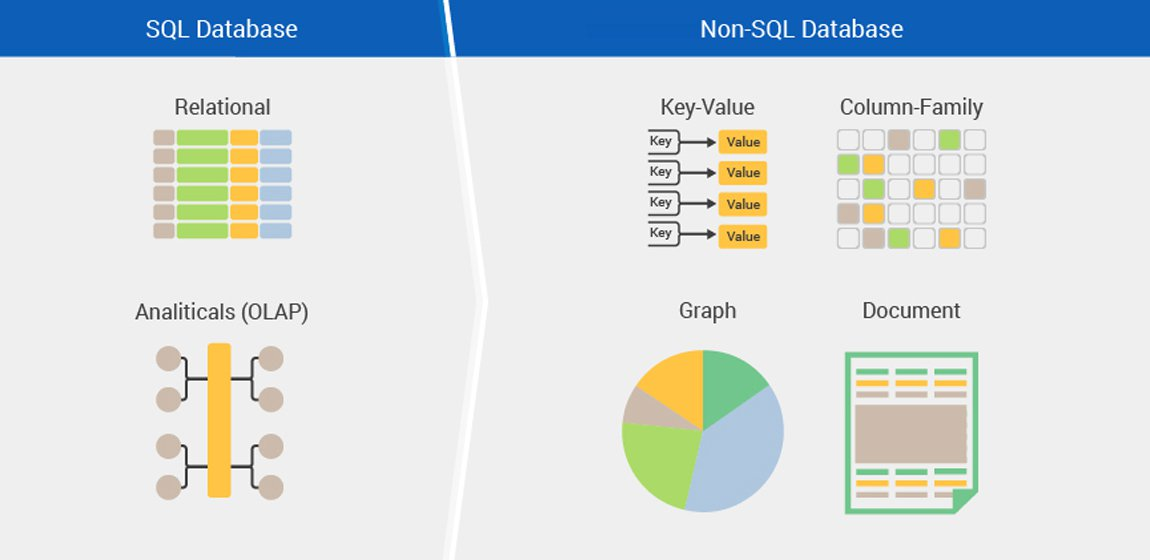
\includegraphics[scale=0.3]{sqlynosql}

\textbf{}\\
\subsection{Formatos}

La información puede organizarse en tablas o en documentos. Cuando organizamos información en un Excel, lo hacemos en formato tabla y, cuando los médicos hacen fichas a sus pacientes, están guardando la información en documentos. Lo habitual es que las bases de datos basadas en tablas sean bases de datos relacionales y las basadas en documentos sean no relacionales, pero esto no tiene que ser siempre así. En realidad, una tabla puede transformarse en documentos, cada uno formado por cada fila de la tabla. Solo es una cuestión de visualización.
\textbf{}\\
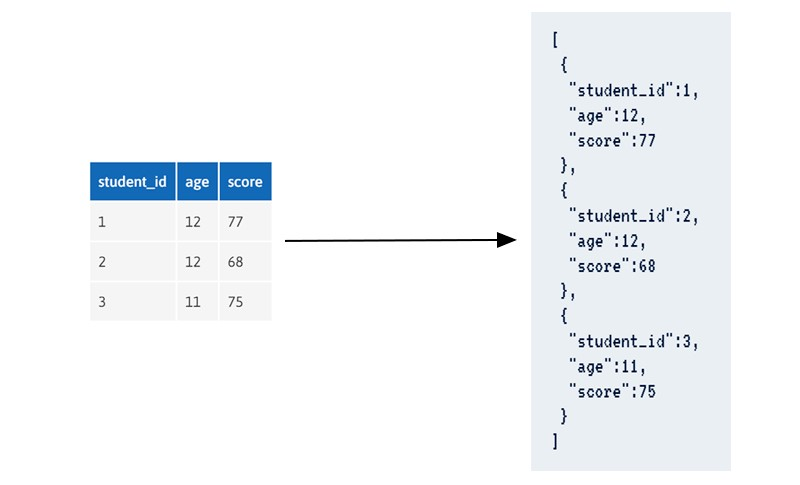
\includegraphics[scale=0.5]{nosql1}
\textbf{}\\
Los dos esquemas de la imagen contienen exactamente la misma información. Lo único que cambia aquí es el formato: cada documento de la figura de la derecha es una fila de la figura de la izquierda.
\textbf{}\\
\textbf{}\\
Se ve más claro en la tabla, ¿verdad? Lo que pasa es que a menudo en una base de datos no relacional una unidad de datos puede llegar a ser demasiado compleja como para plasmarlo en una tabla. \textbf{}\\
\textbf{}\\
\textbf{}\\
Por ejemplo, en el documento JSON de la imagen que se muestra a continuación, al tener elementos jerárquicos, es más difícil plasmarlo en una tabla plana. Una solución sería plasmarlo en varias tablas y, por tanto, necesitar de relaciones.


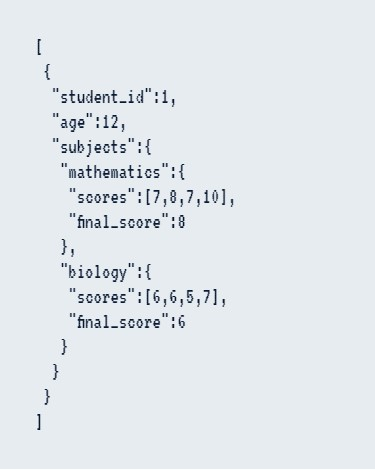
\includegraphics[scale=0.5]{nosql2}

Esto explica por qué las bases de datos relacionales suelen servirse de tablas y las no relacionales de documentos JSON. En cualquier caso, a día de hoy, \textbf{las bases de datos más competitivas suelen permitir, de una forma u otra, operaciones de los dos tipos.}\\ 
\textbf{}\\
 Por ejemplo, el servicio de base de datos en la nube BigQuery que ofrece Google es, en principio, una base de datos de lenguaje de consulta SQL, por lo que permite fácilmente relacionar varias tablas, pero, a su vez, permite insertar elementos jerárquicos JSON, más propios de bases de datos no relacionales.

\textbf{}\\
\textbf{}\\
\textbf{La diferencia entre el éxito y el fracaso recae, sobre todo, en el diseño del modelo.}\\  Es decir, si se decide que el mejor enfoque es usar una base de datos relacional, no es suficiente con meter la información a lo bruto en una base de datos relacional y esperar a que se relacione sola, porque eso no va a ocurrir. De nada sirve elegir la base de datos más apropiada para nuestro sistema, si luego no se hace un buen diseño.

\textbf{}\\
\textbf{}\\



\subsection{Ventajas y Desventajas de SQL y NoSQL}
\textbf{Ventajas de las Bases de Datos relacionales}\\

-	Está más adaptado su uso y los perfiles que las conocen son mayoritarios y más baratos.\\
\textbf{}\\
-	Debido al largo tiempo que llevan en el mercado, estas herramientas tienen un mayor soporte y mejores suites de productos y add-ons para gestionar estas bases de datos.\\
\textbf{}\\
-	La atomicidad de las operaciones en la base de datos. Esto es, que en estas bases de datos o se hace la operación entera o no se hace utilizando la famosa técnica del rollback.\\
\textbf{}\\
-	Los datos deben cumplir requisitos de integridad tanto en tipo de dato como en compatibilidad.\\
\textbf{}\\
\textbf{}\\
\textbf{}\\
\textbf{}\\
\textbf{}\\
\textbf{Desventajas de las Bases de Datos relacionales}\\

-	La atomicidad de las operaciones juega un papel crucial en el rendimiento de las bases de datos.\\
\textbf{}\\
-	Escalabilidad, que aunque probada en muchos entornos productivos suele, por norma, ser inferior a las bases de datos NoSQL.\\

\textbf{}\\
\textbf{-------------------------------------------------------}\\

\textbf{Ventajas de una base de datos NoSQL}\\
\textbf{}\\
-	La escalabilidad y su carácter descentralizado. Soportan estructuras distribuidas.\\
\textbf{}\\

-	Suelen ser bases de datos mucho más abiertas y flexibles. Permiten adaptarse a necesidades de proyectos mucho más fácilmente que los modelos de Entidad Relación.\\
\textbf{}\\

-	Se pueden hacer cambios de los esquemas sin tener que parar bases de datos.\\
\textbf{}\\
-	Escalabilidad horizontal: son capaces de crecer en número de máquinas, en lugar de tener que residir en grandes máquinas.\\
\textbf{}\\
-	Se pueden ejecutar en máquinas con pocos recursos.\\
\textbf{}\\
-	Optimización de consultas en base de datos para grandes cantidades de datos.\\

\textbf{}\\
\textbf{}\\
\textbf{Desventajas de una base de datos NoSQL}\\

-	No todas las bases de datos NoSQL contemplan la atomicidad de las instrucciones y la integridad de los datos. Soportan lo que se llama consistencia eventual.\\
\textbf{}\\
-	Problemas de compatibilidad entre instrucciones SQL. Las nuevas bases de datos utilizan sus propias características en el lenguaje de consulta y no son 100 por ciento compatibles con el SQL de las bases de datos
 relacionales. El soporte a problemas con las queries de trabajo en una base de datos NoSQL es más complicado.
\textbf{}\\
-	Falta de estandarización. Hay muchas bases de datos NoSQL y aún no hay un estándar como sí lo hay en las bases de datos relacionales. Se presume un futuro incierto en estas bases de datos.\\
\textbf{}\\
-	Soporte multiplataforma. Aún quedan muchas mejoras en algunos sistemas para que soporten sistemas operativos que no sean Linux.\\
\textbf{}\\
-	Suelen tener herramientas de administración no muy usables o se accede por consola.\\

\textbf{}\\
\textbf{}\\

\subsection{SQL Vs NoSQL }
\textbf{Cuándo utilizar qué tipo de base de datos}\\
\textbf{}\\
-	Cuando los datos deben ser consistentes sin dar posibilidad al error utilizar una base de datos relacional, SQL.\\
\textbf{}\\
-	Cuando nuestro presupuesto no se puede permitir grandes máquinas y debe destinarse a máquinas de menor rendimiento, NoSQL.\\
\textbf{}\\
-	Cuando las estructuras de datos que manejamos son variables, NoSQL.\\
\textbf{}\\
-	Análisis de grandes cantidades de datos en modo lectura, NoSQL.\\
\textbf{}\\
-	Captura y procesado de eventos, NoSQL.\\
\textbf{}\\
-	Tiendas online con motores de inteligencia complejos, NoSQL.\\
\textbf{}\\

Es muy importante en este punto insistir en que, aunque parece que en estos momentos lo suyo es migrar a bases de datos NoSQL, debemos tener muy en cuenta antes de tomar esta decisión si las características de nuestra base de datos necesitan una base de datos NoSQL o relacional.
Una base de datos NoSQL incluye simplicidad de diseño, escala horizontal más simple para grupos de máquinas y un mejor control de la disponibilidad.

\section{¿Cuándo debería usarse NoSQL?}

Cuando gran cantidad de datos necesitan ser almacenados y recuperados.
La relación entre los datos que almacenas no es tan importante
Los datos cambian con el tiempo y no están estructurados.
No se requiere soporte de restricciones y uniones a nivel de base de datos
Los datos crecen continuamente y usted necesita escalar la base de datos regularmente para manejar los datos.


\textbf{}\\
\textbf{}\\
\textbf{}\\
\section{Conclusiones}
Un NoSQL originalmente referido a no SQL o no relacional es una base de datos que proporciona un mecanismo para el almacenamiento y recuperación de datos. Estos datos se modelan en medios distintos a las relaciones tabulares utilizadas en las bases de datos relacionales. 
Siempre es bueno evaluar las diferentes alternativas que ofrece el mundo del software, para poder dar solución a muchas de los requerimientos que se presentan en el medio, pero siempre hay que considerar que cualquier solución de software que se seleccione va a tener sus ventajas y desventajas al momento de su desarrollo como también en la operación.\textbf{}\\
\textbf{}\\
La aparición del nuevo NoSQL es relativamente nueva, todavía le queda mucho tiempo para poder afirmar si es la solución a muchos de los problemas que hoy en día se presentan en el mundo de la base de datos, una de las ventajas muy importantes que ofrece NoSQL es que puede manejar grandes cantidades de información, pudiendo devolver el resultado de una consulta en cuestión de segundo, cuando un manejador tradicional RDBMS puede tardar 1000 veces mas el tiempo que el anterior haya resuelto. \textbf{}\\
\textbf{}\\
Antes de tomar la decisión de migrar una base de datos relacional a una no relacional hay que considerar todos estos puntos ventajas y desventajas para no caer en un punto del cual ya no se puede regresar y no tener perdidas de información importantes.




\textbf{}\\
\textbf{}\\
%----------------------------------------------------------------------------------------
%	REFERENCE LIST
%----------------------------------------------------------------------------------------

\begin{thebibliography}{99} % Bibliography - this is intentionally simple in this template



\newblock 
1. http://revistatelematica.cujae.edu.cu/
index.php/tele/article/view/23/21
 \break
\newblock 
2. https://programarfacil.com/blog/
que-es-un-orm/
\break
\newblock 
3. https://www.beeva.com/beeva-view/tecnologia/mas-alla-de-la-virtualizacion-contenedores/
\break
\newblock
4. https://searchdatacenter.techtarget.com/
es/definicion/virtualizacion-basada-en-contenedores-virtualizacion-a-nivel-de-sistema-operativo
\break
\newblock
5. https://www.incibe-cert.es/blog/asegurando-virtualizacion-tus-sistemas-control
\break
\newblock
6. http://www.datakeeper.es/?p=716
\break
\newblock
7.https://sigmodrecord.org/publications/sigmodRecord/1012/pdfs/04.surveys.cattell.pdf
\break
\newblock
8.https://ieeexplore.ieee.org/abstract/document/6625441
\break
\newblock
9.-http://nosql-database.org/
\break
\newblock {\em }
 
\end{thebibliography}



%----------------------------------------------------------------------------------------
\end{itemize}
\end{flushright}
\end{document}

